%CAP. 4
\chapter{Resultados e Discussões}
\label{ch:resultados}

\section{Introdução}
Faça uma breve descrição de tudo o que será visto neste capítulo.

\section{Resultados}
Aqui você coloca todos os resultados, experimentos, etc. que você conseguiu com sua proposta. Lembre-se que este capítulo, junto com o Capítulo 3, são os mais importantes. As informações destes capítulos não podem ser encontradas em nenhum outro lugar no mundo pois este é um trabalho original, inédito. Lembre-se de dar o maior número detalhes possível. 

Lembro que em todo o TCC é preciso descrever cada figura e cada tabela no texto. O comentários devem vir no parágrafo anterior à figura ou à tabela em questão. As legendas devem ser concisas e a explicação no parágrafo deve ser completa. É preciso descrever textualmente o conteúdo da figura ou tabela. Se for uma tabela muito longa, focar apenas nos pontos principais. Sempre deve ressaltar os pontos principais. Não assuma que o leitor vai ver a mesma coisa que você ao olhar para a figura ou para a tabela, deixe claro no texto o que você quer mostrar.

A Tabela \ref{tab:exemplo} mostra a notas dos três estudantes utilizados na nossa amostra. Percebe-se claramente que Isabela tem a maior média (9,0). Tanto João quanto Isabela aumentaram suas notas na segunda prova, João foi de 5,0 para 6,0 e Isabela foi de 8,6 para 9,4. Desta fato supõe-se que a Prova 2 estava mais fácil. Já Maria Oliveira teve nota mais baixa na segunda prova, quando se esperava o contrário. Além do mais a nota de Maria foi igual à nota de João. A partir destes dois indícios foi que iniciou a investigação sobre ter havido cópia durante a Prova 2.

\begin{table}
\caption{Notas dos estudantes}
\label{tab:exemplo}
\begin{center}
\renewcommand{\tabcolsep}{2 pt}
\begin{tabular}{ l r r r }
\hline
& \multicolumn{3}{c}{Notas}\\
\cline{2 - 4} % linha horizontal entre as colunas
% 2 e 4
\multicolumn{1}{c}{
\multirow[c]{-2}{*}{Nome}} & Prova 1 & Prova 2 & Média\\
\hline
João Silva & 5{,}0 & 6{,}0 & 5{,}5\\
Maria Oliveira & 7{,}0 & 6{,}0 & 6{,}5\\
Isabela Medeiros & 8{,}6 & 9{,}4 & 9{,}0\\
\hline
\end{tabular}
\end{center}
\end{table}

A Figura \ref{fig:foto} mostra uma foto do canteiro central da UFAPE há mais de 10 anos, quando a árvores ainda era muito pequena. Ao fundo está o prédio da biblioteca, que também contava com sala de aulas e o departamento de informática. Hoje este prédio abriga a reitoria.

\begin{figure}[!htb]
\centering
\caption{Foto do canteiro central da UFAPE}
\label{fig:foto}
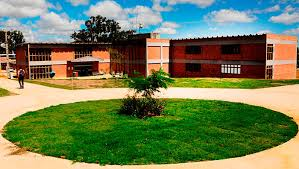
\includegraphics{images/ufape.jpeg}
\end{figure}

Perceba que, ao me referir a uma figura ou tabela específica, trato a figura ou tabela como nome próprio e utilizo letra maiúscula. Isto vale tanto para a Tabela \ref{tab:exemplo} quanto para a Figura \ref{fig:foto}. Mas se falo sem apontar o número utilizo letra minúscula para me referir àquela tabela ou a esta figura.

O mesmo vale para equações. Quando me referir a uma equação importante devo utilizar seu número. Por exemplo, a Equação \ref{eq:segundo_grau} é uma equação do segundo grau:
\begin{equation}
f(x) = ax^2 + bx + c,
\label{eq:segundo_grau}
\end{equation}
esta equação associa um função $f$ de $x$ com um polinômio do segundo grau. $a$, $b$ e $c$, são constantes que dão o peso de cada parte da equação. $a$ indica a contribuição de $x^2$, $b$ a contribuição de $x$ e, finalmente, $c$ é uma contante somada ao todo (pode ser interpretada como contribuição do 1).
Cada equação deve ser descrita, explicando o que é cada elemento dela.
Veja que a equação termina com um vírgula (poderia terminar com um ponto final). Deve-se utilizar a pontuação na equação como se ela fosse uma palavra do texto.

\section{Discussão}
A discussão pode vir na junto dos resultados, separado ou ambos (uma parte com os resultados e outra depois). A discussão é uma interpretação dos resultados, uma ``tradução''. É preciso deixar claro quais são os resultados. 
Na discussão também comparar seus resultados com os resultados de outros autores. As possibilidades são inúmeras e vai depender da sua análise.

\section{Considerações Finais}
Faça uma recapitulação do que foi visto neste capítulo. E termine fazendo uma conexão com o que será visto no capítulo seguinte.